\documentclass[serif, xcolor=dvipsnames]{beamer}

\makeatletter

% HAY QUE ELEGIR EL QUE CORRESPONDA

% \usepackage{mathpazo}%Letra palatino con fuentes para matemáticas
\usepackage[T1]{fontenc}
\usepackage[utf8]{inputenc}
\usepackage{graphicx}
\usepackage{url}
\usepackage{amsmath}
\usepackage{booktabs}
\usepackage{textcomp}%%needed for the euro symbol

\date{}

\usepackage[emulate=units]{siunitx}
\sisetup{per=fraction, fraction=nice, decimalsymbol=comma}
\newunit{\wattpeak}{Wp}
\newunit{\watthour}{Wh}
\newunit{\amperehour}{Ah}

\setbeamercovered{transparent}
\setbeamertemplate{navigation symbols}{}
\usefonttheme{structuresmallcapsserif} 
\usefonttheme{serif} 
\usefonttheme{structurebold}

%\usepackage{epstopdf}


\usepackage[spanish]{babel}
\addto\shorthandsspanish{\spanishdeactivate{~<>}}

\hypersetup{pdfauthor={Oscar Perpi\~n\'an},%
    pdftitle={Energ\'ia Solar Fotovoltaica},%
    filecolor=blue,%
    urlcolor=blue}



%\usepackage{handoutWithNotes} %para hacer papel con notas 
%\pgfpagesuselayout{4 on 1 with notes}[a4paper,border shrink=5mm]



%\usepackage{pgfpages}
%\pgfpagesuselayout{2 on 1}[a4paper,border shrink=5mm]

 
% \usepackage{mathpazo}%Letra palatino con fuentes para matemáticas
\usepackage[T1]{fontenc}
\usepackage[utf8]{inputenc}
\usepackage{graphicx}
\usepackage{url}
\usepackage{amsmath}
\usepackage{booktabs}

\usepackage[spanish]{babel}
\addto\shorthandsspanish{\spanishdeactivate{~<>}}


\usepackage{hyperref}
% \hypersetup{pdfauthor={Oscar Perpi\~n\'an},%
%     pdftitle={Energ\'ia Solar Fotovoltaica},%
%     filecolor=blue,%
%     urlcolor=blue}

\hypersetup{
    bookmarks=true,         % show bookmarks bar?
%    unicode=true,          % non-Latin characters in Acrobat’s bookmarks
    bookmarksnumbered=false,
    bookmarksopen=false,
    breaklinks=true,
    backref=true,
    pdftoolbar=true,        % show Acrobat’s toolbar?
    pdfmenubar=true,        % show Acrobat’s menu?
    pdffitwindow=false,     % window fit to page when opened
    pdfstartview={FitH},    % fits the width of the page to the window
    pdftitle={Energía Solar Fotovoltaica},    % title
    pdfauthor={Oscar Perpiñán Lamigueiro},     % author
    pdfsubject={Electrotecnia},   % subject of the document
    pdfcreator={AucTeX/Emacs},   % creator of the document
    pdfproducer={LaTeX}, % producer of the document
    pdfnewwindow=true,      % links in new window
    pdfborder={0 0 0},
    colorlinks=true,       % false: boxed links; true: colored links
    linkcolor=,          % color of internal links
    citecolor=BrickRed,        % color of links to bibliography
    filecolor=black,      % color of file links
    urlcolor=Blue           % color of external links 
}

\usepackage[emulate=units]{siunitx}
\sisetup{per=fraction, fraction=nice, decimalsymbol=comma}
\newunit{\wattpeak}{Wp}
\newunit{\watthour}{Wh}
\newunit{\amperehour}{Ah}

\setbeamercovered{transparent}
\setbeamertemplate{navigation symbols}{}
\usefonttheme{serif} 
\usefonttheme{structuresmallcapsserif} 

\useinnertheme[shadow=true]{rounded}
\useoutertheme{shadow}
%\usecolortheme[named=BrickRed]{structure} %sirve para cambiar el color genérico
\usecolortheme{orchid}
\usecolortheme{whale}
\documentclass[xcolor={usenames,svgnames,dvipsnames}]{beamer}
\usepackage[utf8]{inputenc}
\usepackage[T1]{fontenc}
\usepackage{graphicx}
\usepackage{grffile}
\usepackage{longtable}
\usepackage{wrapfig}
\usepackage{rotating}
\usepackage[normalem]{ulem}
\usepackage{amsmath}
\usepackage{textcomp}
\usepackage{amssymb}
\usepackage{capt-of}
\usepackage{hyperref}
\usepackage{color}
\usepackage{listings}
\usepackage{mathpazo}
\usepackage{gensymb}
\usepackage{amsmath}
\usepackage{chemarr}%flechas para reacciones químicas (SFER.tex)
\bibliographystyle{plain}
\AtBeginSubsection[]{\begin{frame}[plain]\tableofcontents[currentsubsection,sectionstyle=show/shaded,subsectionstyle=show/shaded/hide]\end{frame}}
\AtBeginSection[]{\begin{frame}[plain]\tableofcontents[currentsection,hideallsubsections]\end{frame}}
\usepackage[emulate=units]{siunitx}
\sisetup{fraction=nice, decimalsymbol=comma, retain-unity-mantissa = false}
\newunit{\wattpeak}{Wp}
\newunit{\watthour}{Wh}
\newunit{\amperehour}{Ah}
\usepackage{steinmetz}
\hypersetup{colorlinks=true, linkcolor=OliveGreen, urlcolor=Blue}
\renewcommand{\thefootnote}{\fnsymbol{footnote}}
\beamertemplatenavigationsymbolsempty
\setbeamertemplate{footline}[frame number]

\setbeamercolor{alerted text}{fg=Green!50!black} \setbeamerfont{alerted text}{series=\bfseries}
\usefonttheme{serif}
\setbeamercovered{transparent}
\setbeamertemplate{navigation symbols}{}
\usefonttheme{serif} 

\setbeamercolor{palette primary}{bg=OliveGreen,fg=white}
\setbeamercolor{palette secondary}{bg=OliveGreen,fg=white}
\setbeamercolor{palette tertiary}{bg=OliveGreen,fg=white}
\setbeamercolor{palette quaternary}{bg=OliveGreen,fg=white}
\setbeamercolor{structure}{fg=OliveGreen} % itemize, enumerate, etc
\setbeamercolor{section in toc}{fg=OliveGreen} % TOC sections

\usetheme[hideothersubsections]{Goettingen}

\usepackage{tikz}

\titlegraphic{
\includegraphics[width=2.5cm]{../figs/logoEOI.jpg}}
\addtobeamertemplate{frametitle}{}{%
\begin{tikzpicture}[remember picture,overlay]
\node[anchor=south east,yshift=2pt] at (current page.south east) {
\includegraphics[width=1.5cm]{../figs/logoEOI.jpg}};
\end{tikzpicture}}

\makeatother


\begin{document}

\title[\textsc{EPBT}]{\textsc{Tiempo de Retorno Energético}\\
  \textsc{de Sistemas Fotovoltaicos}}


\author{\textsc{Oscar Perpiñán Lamigueiro}}

\date{}

\frame[plain]{\titlepage}

\selectlanguage{spanish}%

\begin{frame}
  \frametitle{Introducción} A lo largo de su ciclo de vida, además de
  producir energía y diferentes residuos, un sistema generador
  requerirá el empleo de energía para:
  \begin{itemize}
  \item Fabricación de componentes
  \item Tratamiento del terreno
  \item Transporte e instalación de los equipos
  \item Combustible necesario para su funcionamiento
  \item Reposición de equipos que agotan su ciclo
  \item ...
  \end{itemize}
\end{frame}

\begin{frame}
  \frametitle{Ciclo de Vida}

  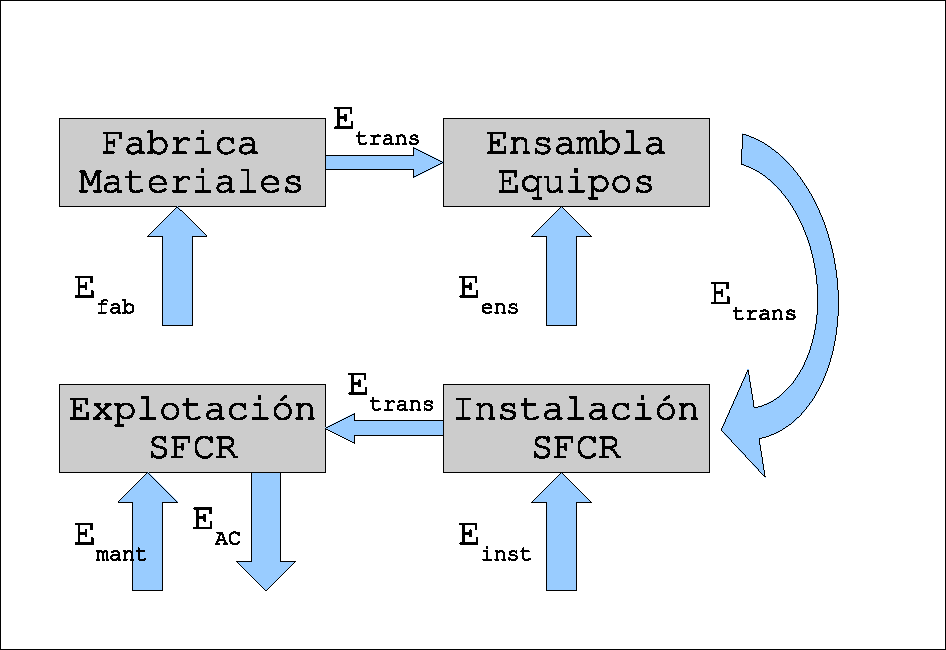
\includegraphics[width=\textwidth]{../Figuras/LCAFlujo}
  
\end{frame}

\begin{frame}
  \frametitle{Fuentes de Información}
  \begin{itemize}
  \item \textbf{Inventarios de Ciclos de Vida} (\emph{Life Cycle
      Inventory,} LCI) de los procesos empleados para implementar un
    SFCR. A partir de estos LCIs es posible estimar el impacto
    energético asociado.
    \begin{itemize}
    \item Incertidumbre alta en módulos FV (40\%)
    \end{itemize}
  \item \textbf{Radiación global} del lugar en el que el SFCR va a
    desempeñar sus funciones
  \item \textbf{Características técnicas de los diferentes
      componentes} del SFCR que permitan estimar la energía producida
    a lo largo de toda su vida útil.
  \end{itemize}
 
\end{frame}


\begin{frame}
  \frametitle{Energy PayBack Time}
  \begin{columns}
    \begin{column}{7cm}
      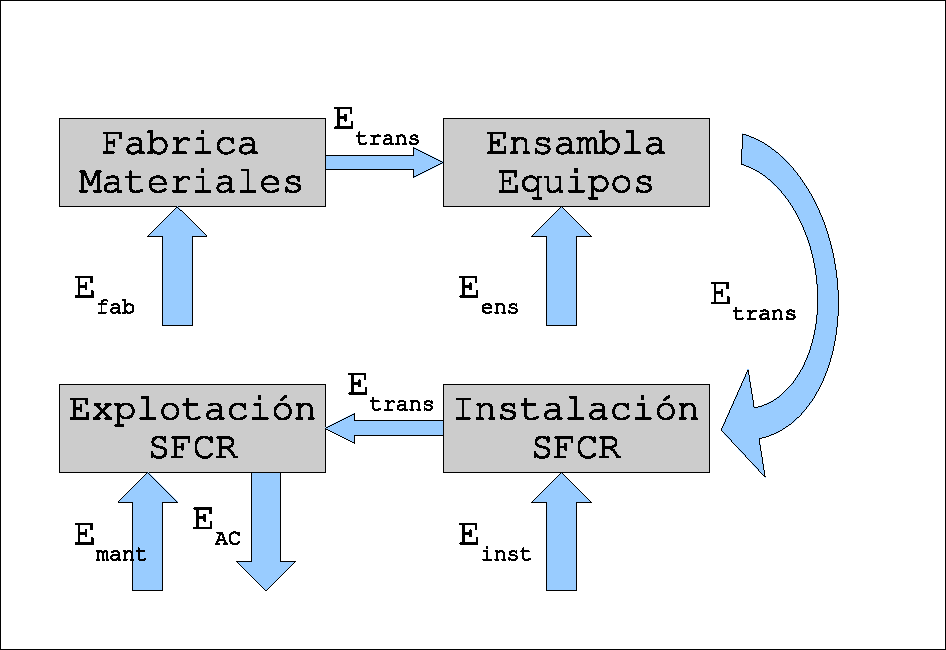
\includegraphics[width=\textwidth]{../Figuras/LCAFlujo}
    \end{column}
    \begin{column}{3cm}
      \begin{equation*}
        EPBT=\frac{E_{LCA}}{E_{ac}}
      \end{equation*}
    \end{column}
  \end{columns}
\end{frame}

\begin{frame}
  \frametitle{La cuestión del mix energético}
  \begin{itemize}
  \item \textbf{La energía primaria depende de la eficiencia de conversión del
    sistema energético.}
    \begin{itemize}
    \item La eficiencia depende de la composición de fuentes
      energéticas (mix energético)
    \item Eficiencia para zona UCTE: 0.31
    \end{itemize}
  \item \textbf{Proceso productivo de módulo FV es principalmente eléctrico}
    (80\% de energía primaria se emplea en electricidad).
    \begin{itemize}
    \item Centros de fabricación en zonas con alta eficiencia de
      conversión.
    \item Menor impacto ambiental con alta penetración de renovables.
    \end{itemize}
  \item La \textbf{producción de la energía eléctrica} del SFCR se produce normalmente \textbf{lejos del
    centro de fabricación} 
    \begin{itemize}
    \item Diferente eficiencia de conversión por variación de mix
      energético.
    \item Menor EPBT inyectando en sistemas poco eficientes.
    \end{itemize}
  \end{itemize}

\end{frame}


\begin{frame}
  \frametitle{Energía de los principales componentes}
  \framesubtitle{Seguimiento a Doble Eje}
  \begin{tabular}{lll}
    \toprule
    Componente              &  ($MJ_{p}/kWp$)  &  (\%)     \\
    \midrule
    Módulo & 41\,819 & 69,54\% \\
    Estructura Soporte      &  9\,329          &  15,51\%  \\
    Mecanismos de seguimiento    &  248             &  0,41\%   \\
    Cimientos (acero)     &  3\,371          &  5,61\%   \\
    Cimientos (hormigón)  &  2\,445          &  4,07\%   \\
    Transporte              &  1\,339          &  2,23\%   \\
    Inversor               &  1,091           &  1,81\%   \\
    Cableado                 &  497             &  0,83\%   \\
    \midrule
    Total                  &  60\,140         &  100\%    \\
    \bottomrule
  \end{tabular}

\end{frame}

\begin{frame}
  \frametitle{Energía de los principales componentes}
  \framesubtitle{Seguimiento de Eje Horizontal NS}
  \begin{tabular}{lll}
    \toprule
    Componente              &  ($MJ_{p}/kWp$)  &  (\%)     \\
    \midrule
    Módulo & 41\,819 & 78,67\% \\
    Estructura Soporte      &  6\,108          &  11,49\%  \\
    Mecanismos de seguimiento    &  58              &  0,11\%   \\
    Cimientos (acero)     &  1\,536          &  2,89\%   \\
    Cimientos (hormigón)  &  1\,281          &  2,41\%   \\
    Transporte              &  900             &  1,69\%   \\
    Inversor               &  1\,091          &  2,05\%   \\
    Cableado                 &  364             &  0,68\%   \\
    \midrule
    Total                  &  53\,157         &  100\%    \\
    \bottomrule
  \end{tabular}
\end{frame}

\begin{frame}
  \frametitle{Energía de los principales componentes}
  \framesubtitle{Sistemas Estáticos}
  \begin{tabular}{lll}
    \toprule
    Componente              &  ($MJ_{p}/kWp$)  &  (\%)    \\
    \midrule
    Módulo & 41\,819 & 81,99\% \\
    Estructura Soporte      &  4\,459          &  8,74\%  \\
    Mecanismos de seguimiento    &  0               &  0,00\%  \\
    Cimientos (acero)     &  0               &  0,00\%  \\
    Cimientos (hormigón)  &  2\,352          &  4,61\%  \\
    Transporte              &  1\,037          &  2,03\%  \\
    Inversor               &  1\,091          &  2,14\%  \\
    Cableado                 &  248             &  0,49\%  \\
    \midrule
    Total                  &  51\,005         &  100\%   \\
    \bottomrule
  \end{tabular}
\end{frame}

\begin{frame}
  \frametitle{Valores de EPBT por sistema}
  \begin{tabular}{ccccccc}
    \toprule
    EPBT & 1st. Quartile & Median & Mean & 3rd Quartile \tabularnewline
    \midrule 
    Doble Eje & 2,4 & 2,6 & 2,7 & 2,82\tabularnewline
    Horizontal-NS &  2,65 & 2,88 & 3 & 3,17\tabularnewline
    Estático & 3 & 3,22 & 3,3 & 3,45\tabularnewline
    \bottomrule 
  \end{tabular}

\end{frame}

\begin{frame}
  \frametitle{Doble Eje}
  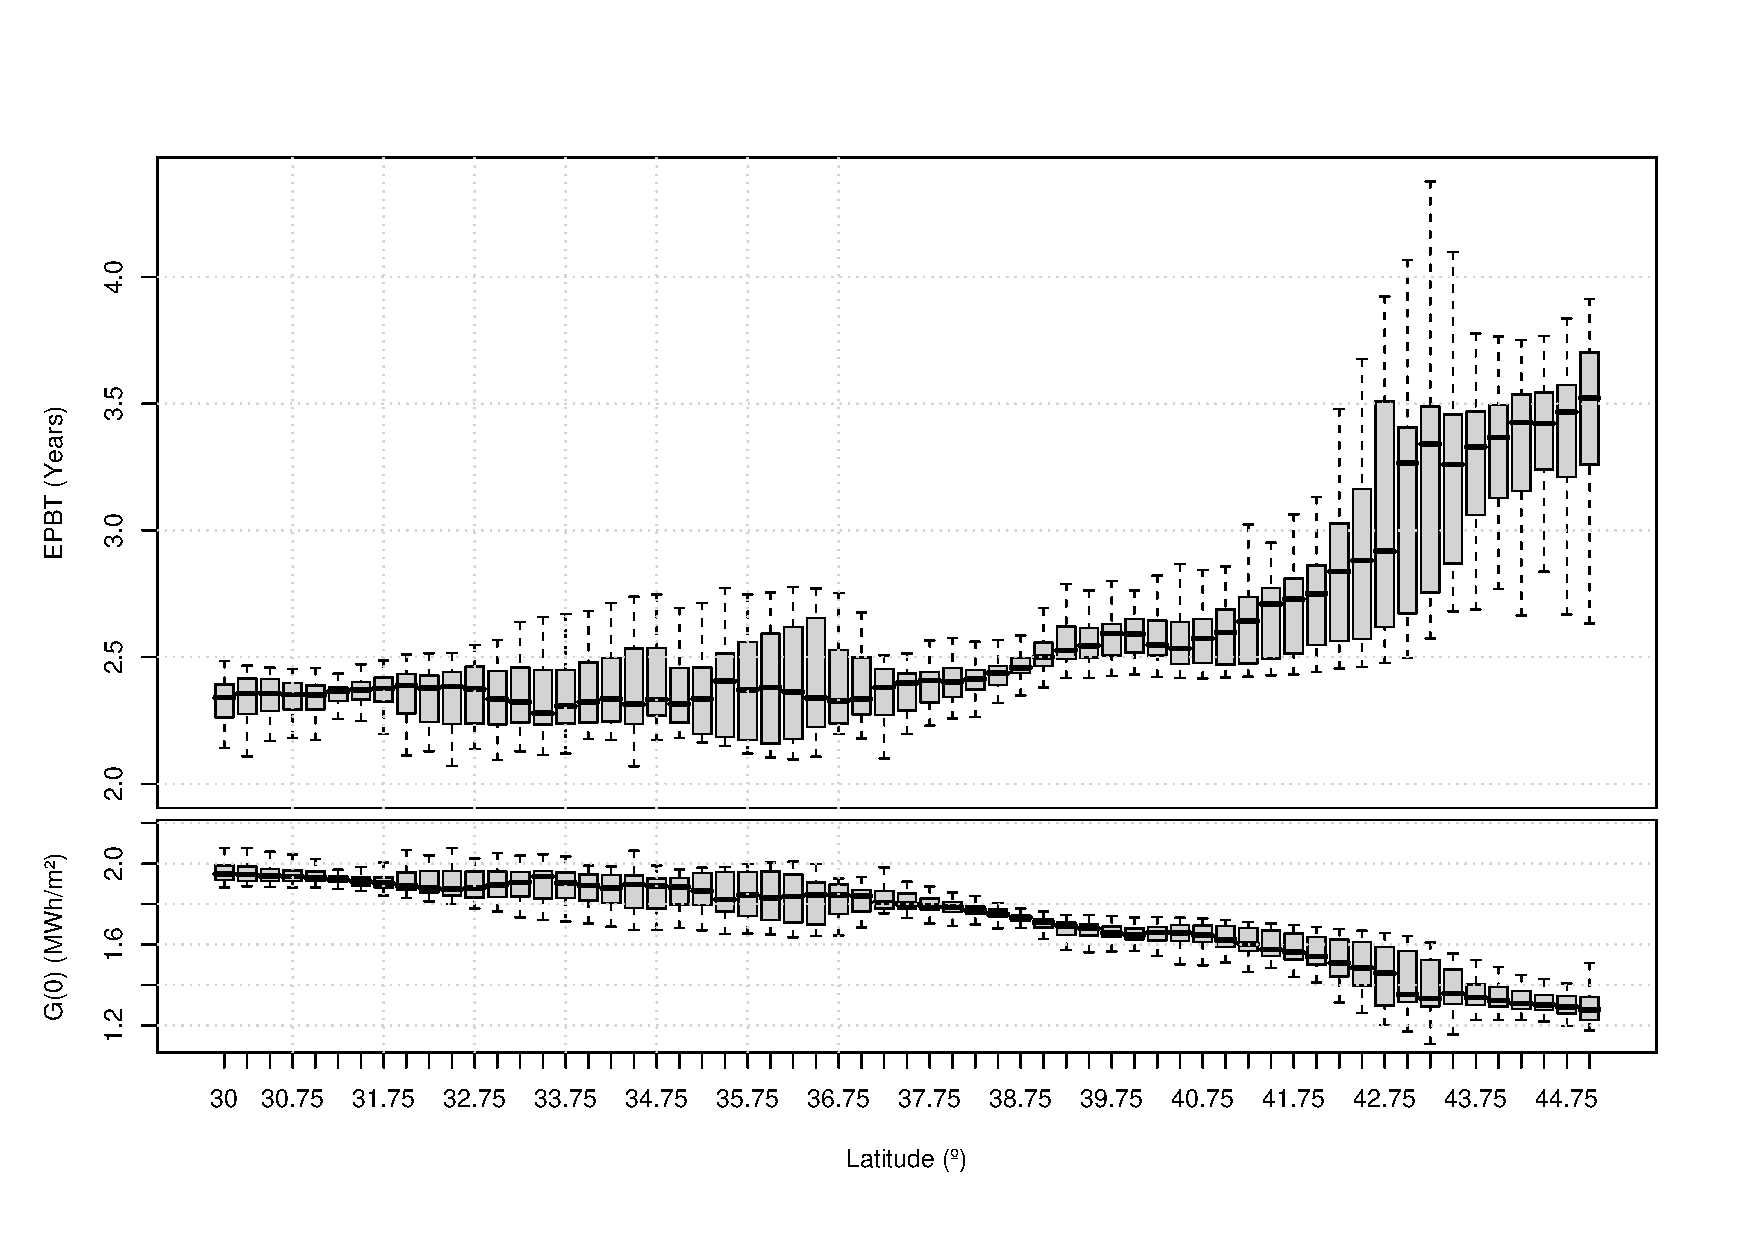
\includegraphics[width=\textwidth]{../Figuras/BoxPlotEPBTEuropa_2x}
\end{frame}

\begin{frame}
  \frametitle{Horizontal NS}
  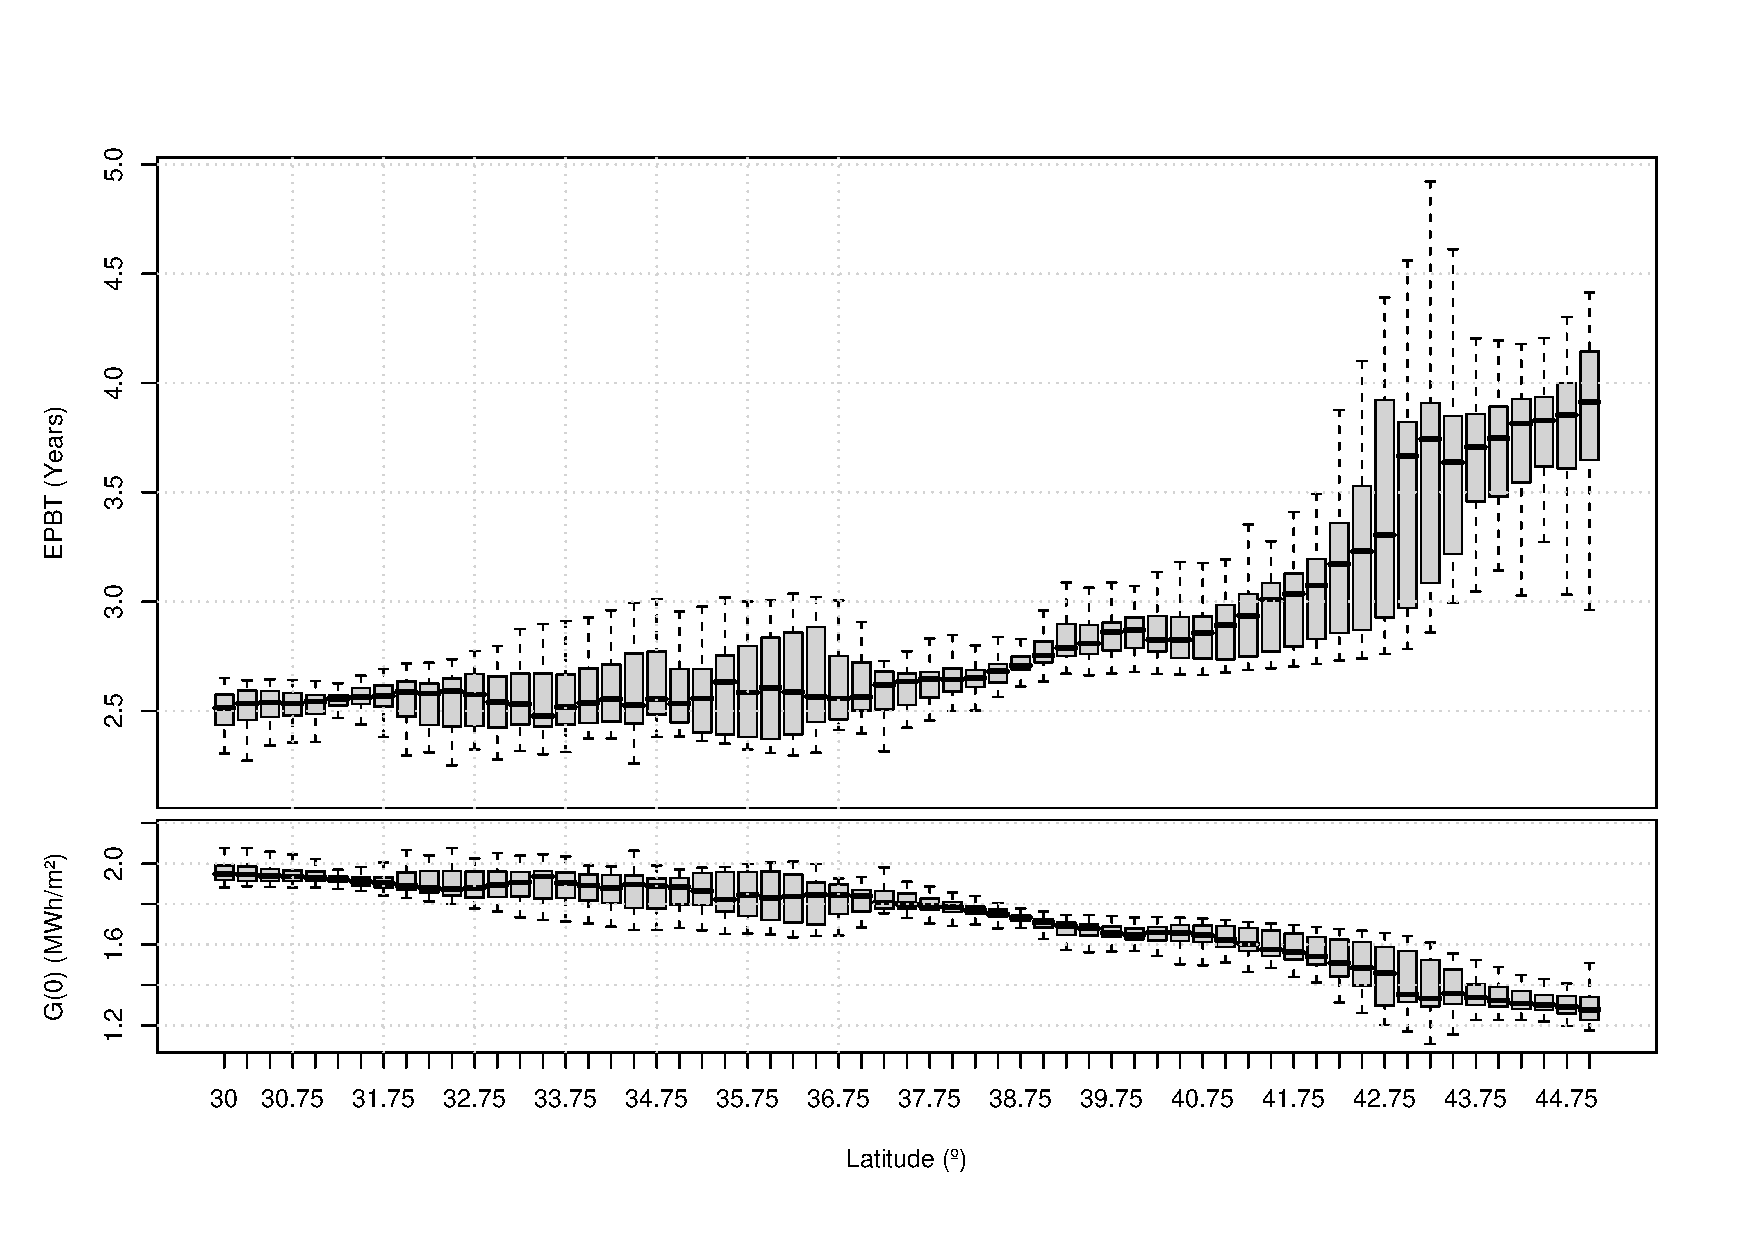
\includegraphics[width=\textwidth]{../Figuras/BoxPlotEPBTEuropa_HorizNS}
\end{frame}

\begin{frame}
  \frametitle{Estático}
  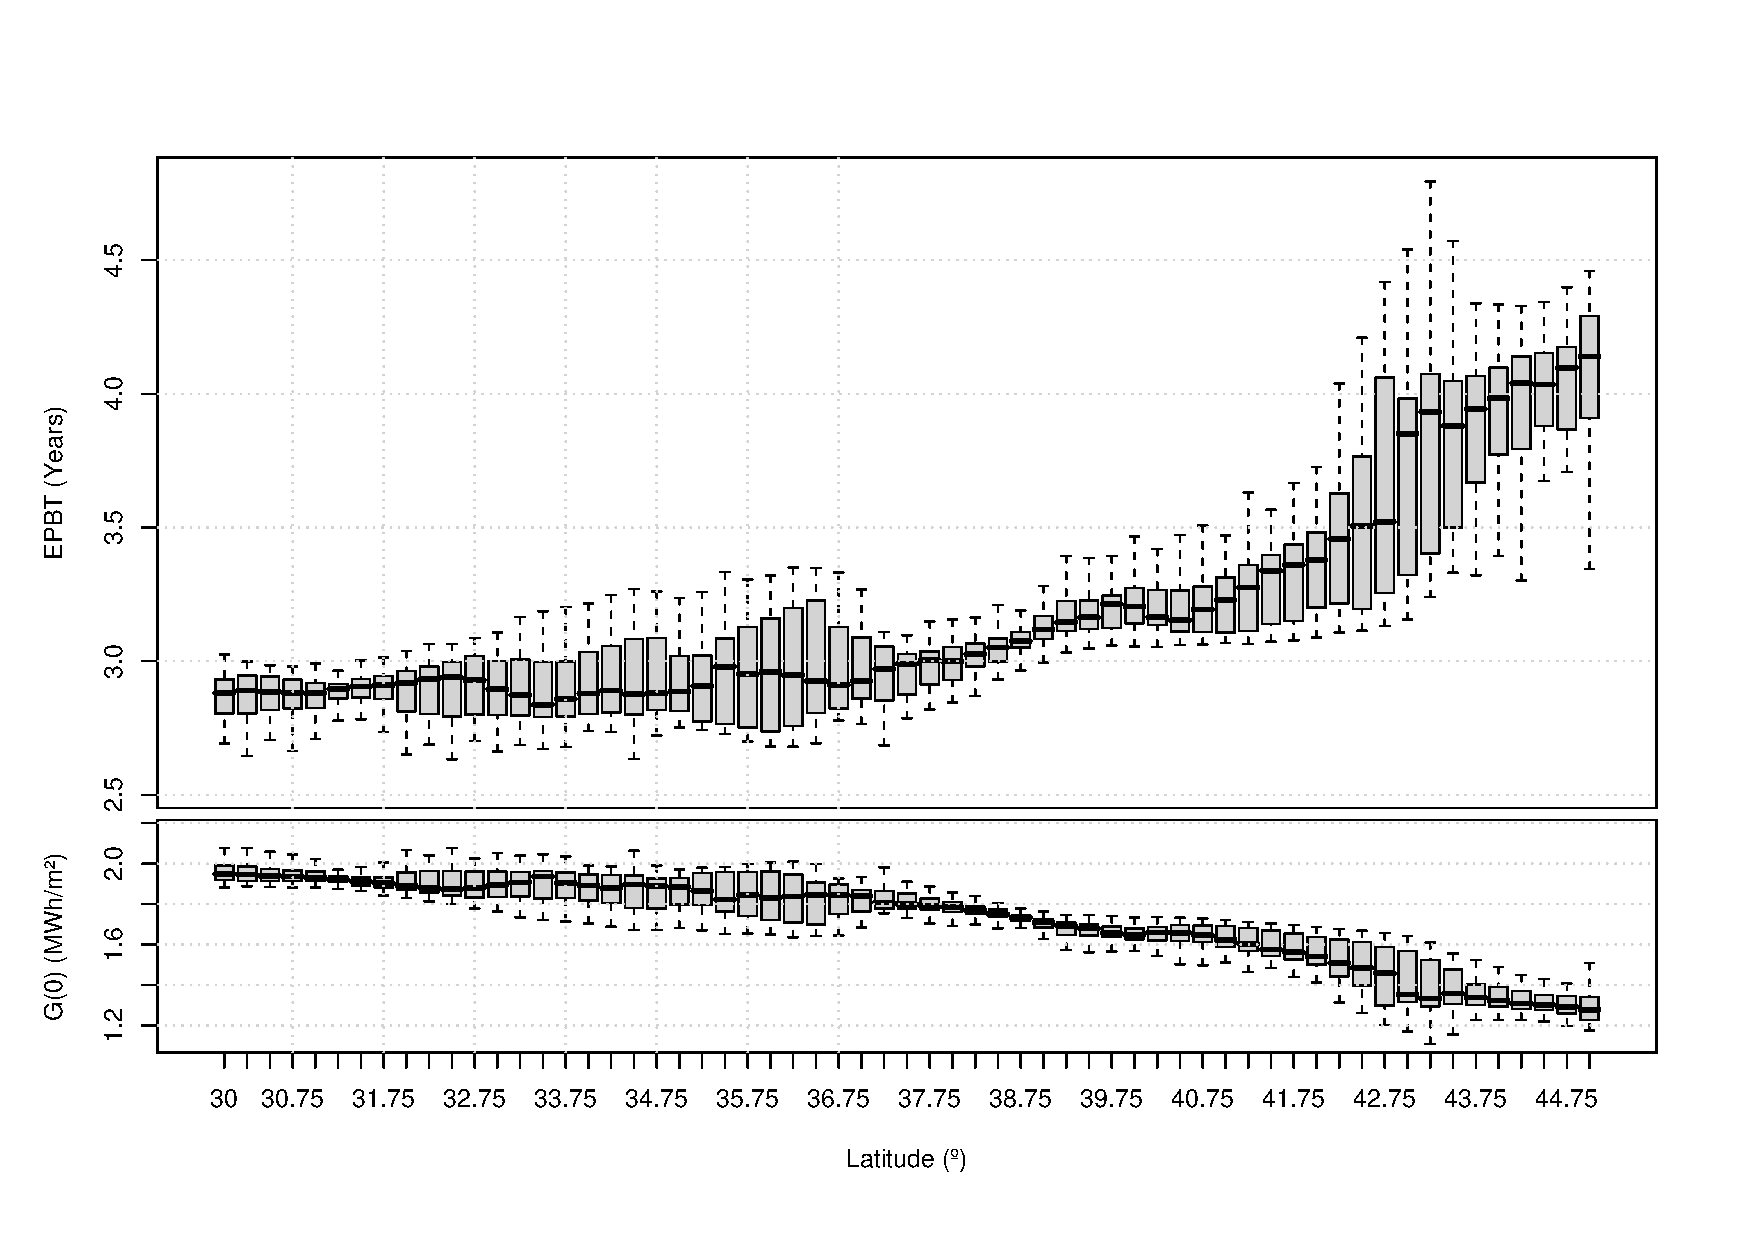
\includegraphics[width=\textwidth]{../Figuras/BoxPlotEPBTEuropa_Fixed}
\end{frame}

\begin{frame}
  \frametitle{Comparativa}
  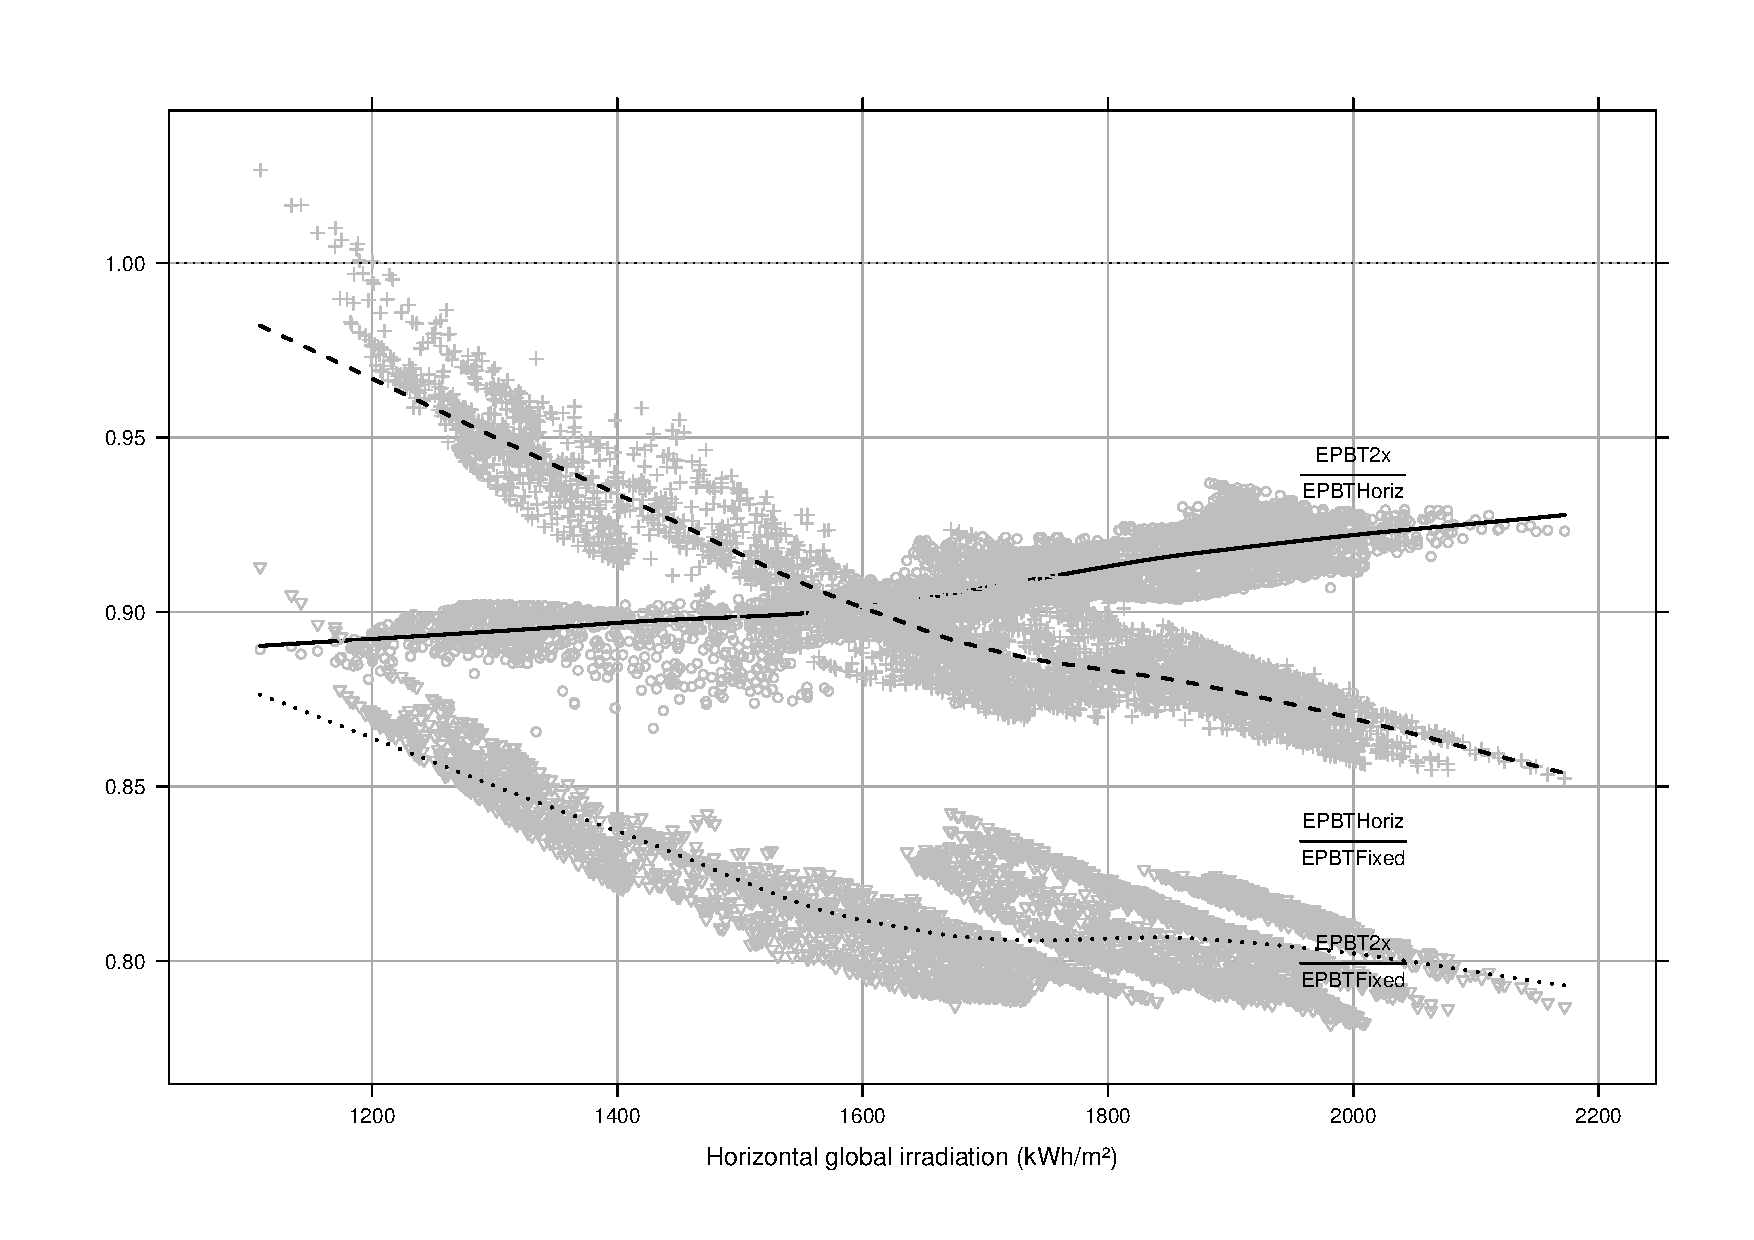
\includegraphics[width=\textwidth]{../Figuras/EPBTEuropavsGh2}
\end{frame}

\end{document}